% LACE method overview figure. Build: tectonic lace_overview.tex  (from this directory)
% Included by paper.tex as figs/lace_overview.pdf
\documentclass[tikz,border=3pt]{standalone}
\usepackage[T1]{fontenc}
\usepackage[scaled=0.92]{helvet}
\renewcommand{\familydefault}{\sfdefault}
\usepackage{amsmath,amssymb}
\usetikzlibrary{positioning,arrows.meta,calc,fit,backgrounds}

% palette
\definecolor{ink}{HTML}{2B2B2B}
\definecolor{frz}{HTML}{3B6EA8}  % frozen
\definecolor{trn}{HTML}{D9822B}  % trained on boxes
\definecolor{ffit}{HTML}{3F8F5F}  % training-free fit from boxes
\definecolor{soil}{HTML}{E9DCC4}
\definecolor{crown}{HTML}{5E9E4E}
\definecolor{crownd}{HTML}{3A6F2E}
\definecolor{ph1}{HTML}{C9D8EC}
\definecolor{ph2}{HTML}{9DBBDD}
\definecolor{ph3}{HTML}{6F9BCB}
\definecolor{ph4}{HTML}{3B6EA8}
\definecolor{panel}{HTML}{F7F7F7}

\tikzset{
  panel/.style={draw=ink!25, fill=panel, rounded corners=4pt, line width=0.4pt, inner sep=6pt},
  title/.style={font=\small\bfseries, text=ink, anchor=north, align=center},
  lbl/.style={font=\scriptsize, text=ink!85, align=center, inner sep=1pt},
  tag/.style={font=\tiny\bfseries, text=white, rounded corners=2pt, inner sep=1.5pt, inner xsep=3pt, anchor=north},
  arr/.style={-{Stealth[length=5pt,width=4pt]}, line width=0.7pt, ink!75},
  sup/.style={-{Stealth[length=4pt,width=3.5pt]}, line width=0.5pt, ink!60},
  supd/.style={sup, dashed},
  box/.style={draw=trn, line width=0.7pt},
}

\begin{document}
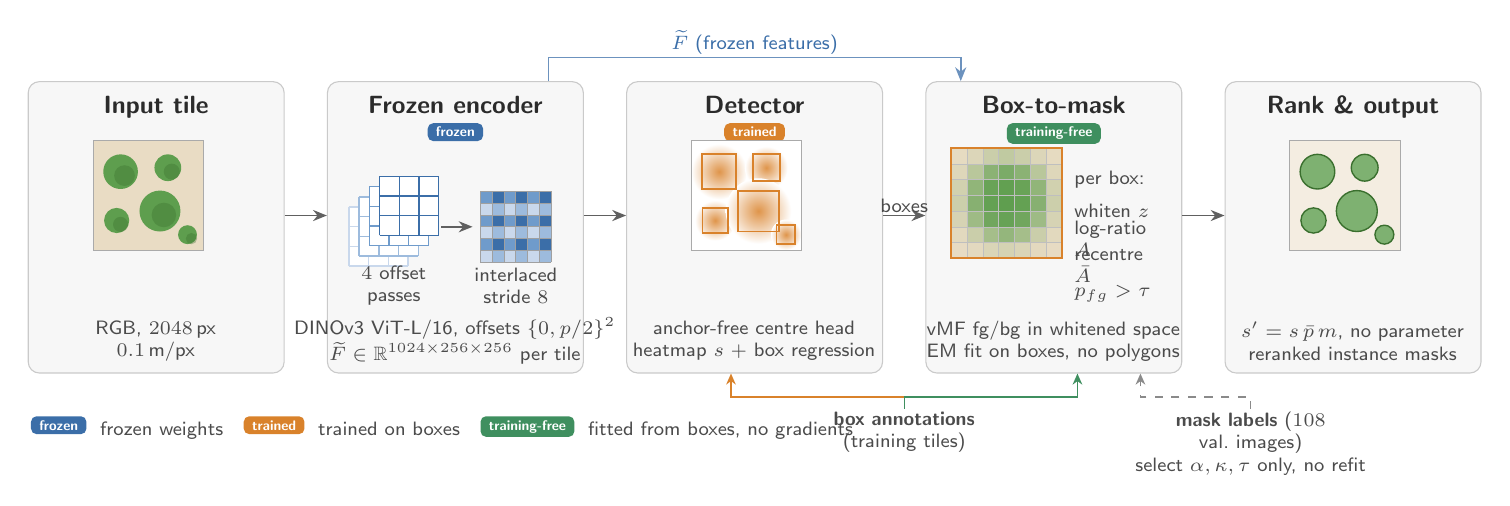
\begin{tikzpicture}[x=1cm,y=1cm]

% ---------------------------------------------------------------- geometry
\def\pw{3.25}      % panel width
\def\gap{0.55}     % gap between panels
\def\ptop{0}       % panel top y
\def\pbot{-3.55}   % panel bottom y

% panel anchors (left x)
\pgfmathsetmacro{\pAx}{0}
\pgfmathsetmacro{\pBx}{\pAx+\pw+\gap}
\pgfmathsetmacro{\pCx}{\pBx+\pw+\gap}
\pgfmathsetmacro{\pDx}{\pCx+\pw+\gap}
\pgfmathsetmacro{\pEx}{\pDx+\pw+\gap}

\foreach \x/\n in {\pAx/A,\pBx/B,\pCx/C,\pDx/D,\pEx/E}{
  \node[panel, minimum width=\pw cm, minimum height=3.7cm, anchor=north west] (P\n) at (\x,\ptop) {};
}

% ---------------------------------------------------------------- A: input
\node[title] at ([yshift=-2pt]PA.north) {Input tile};
\begin{scope}[shift={(\pAx+0.83,-2.15)}]
  \fill[soil] (0,0) rectangle (1.4,1.4);
  \foreach \cx/\cy/\r in {0.35/1.0/0.22, 0.95/1.05/0.17, 0.3/0.38/0.16, 0.85/0.5/0.26, 1.2/0.2/0.12}{
    \fill[crown] (\cx,\cy) circle (\r);
    \fill[crownd, opacity=0.35] (\cx+0.05,\cy-0.05) circle (0.6*\r);
  }
  \draw[ink!40, line width=0.3pt] (0,0) rectangle (1.4,1.4);
\end{scope}
\node[lbl] at (\pAx+0.5*\pw,-3.3) {RGB, $2048$\,px\\$0.1$\,m/px};

% ---------------------------------------------------------------- B: encoder
\node[title] at ([yshift=-2pt]PB.north) {Frozen encoder};
\node[tag, fill=frz] at ([yshift=-15pt]PB.north) {frozen};
% four offset 3x3 grids
\begin{scope}[shift={(\pBx+0.28,-2.35)}]
  \foreach \i/\c in {0/ph1,1/ph2,2/ph3,3/ph4}{
    \begin{scope}[shift={(0.13*\i,0.13*\i)}]
      \fill[white] (0,0) rectangle (0.75,0.75);
      \draw[\c, line width=0.5pt, step=0.25] (0,0) grid (0.75,0.75);
    \end{scope}
  }
\end{scope}
\node[lbl] at (\pBx+0.85,-2.6) {$4$ offset\\passes};
% arrow
\draw[arr] (\pBx+1.45,-1.85) -- (\pBx+1.85,-1.85);
% interlaced 6x6 grid, 2x2 colour tiling
\begin{scope}[shift={(\pBx+1.95,-2.3)}]
  \foreach \i in {0,...,5}{ \foreach \j in {0,...,5}{
    \pgfmathtruncatemacro{\pi}{mod(\i,2)+2*mod(\j,2)}
    \ifcase\pi \def\c{ph1}\or\def\c{ph2}\or\def\c{ph3}\else\def\c{ph4}\fi
    \fill[\c] (0.15*\i,0.15*\j) rectangle ++(0.15,0.15);
  }}
  \draw[ink!45, line width=0.3pt, step=0.15] (0,0) grid (0.9,0.9);
\end{scope}
\node[lbl] at (\pBx+2.4,-2.6) {interlaced\\stride $8$};
\node[lbl] at (\pBx+0.5*\pw,-3.3) {DINOv3 ViT-L/16, offsets $\{0,p/2\}^2$\\$\widetilde F \in \mathbb{R}^{1024\times256\times256}$ per tile};

% ---------------------------------------------------------------- C: detector
\node[title] at ([yshift=-2pt]PC.north) {Detector};
\node[tag, fill=trn] at ([yshift=-15pt]PC.north) {trained};
\begin{scope}[shift={(\pCx+0.83,-2.15)}]
  \fill[white] (0,0) rectangle (1.4,1.4);
  \foreach \cx/\cy/\r in {0.35/1.0/0.22, 0.95/1.05/0.17, 0.3/0.38/0.16, 0.85/0.5/0.26, 1.2/0.2/0.12}{
    \shade[inner color=trn!85, outer color=white] (\cx,\cy) circle (1.6*\r);
  }
  \foreach \cx/\cy/\r in {0.35/1.0/0.22, 0.95/1.05/0.17, 0.3/0.38/0.16, 0.85/0.5/0.26, 1.2/0.2/0.12}{
    \draw[box] (\cx-\r,\cy-\r) rectangle (\cx+\r,\cy+\r);
  }
  \draw[ink!40, line width=0.3pt] (0,0) rectangle (1.4,1.4);
\end{scope}
\node[lbl] at (\pCx+0.5*\pw,-3.3) {anchor-free centre head\\heatmap $s$ + box regression};

% ---------------------------------------------------------------- D: box-to-mask
\node[title] at ([yshift=-2pt]PD.north) {Box-to-mask};
\node[tag, fill=ffit] at ([yshift=-15pt]PD.north) {training-free};
% one box, cells coloured by posterior
\begin{scope}[shift={(\pDx+0.33,-2.25)}]
  \foreach \i in {0,...,6}{ \foreach \j in {0,...,6}{
    \pgfmathsetmacro{\dd}{sqrt((\i-3)^2+(\j-3.2)^2)}
    \pgfmathsetmacro{\pp}{100/(1+exp(2.2*(\dd-2.4)))}
    \fill[crown!\pp!soil] (0.2*\i,0.2*\j) rectangle ++(0.2,0.2);
  }}
  \draw[ink!30, line width=0.2pt, step=0.2] (0,0) grid (1.4,1.4);
  \draw[box] (0,0) rectangle (1.4,1.4);
\end{scope}
\node[lbl, anchor=west, align=left] at (\pDx+1.85,-1.25) {per box:};
\node[lbl, anchor=west, align=left, text width=1.15cm] at (\pDx+1.85,-1.65) {whiten $z$};
\node[lbl, anchor=west, align=left, text width=1.15cm] at (\pDx+1.85,-2.00) {log-ratio $A$};
\node[lbl, anchor=west, align=left, text width=1.15cm] at (\pDx+1.85,-2.35) {recentre $\bar A$};
\node[lbl, anchor=west, align=left, text width=1.15cm] at (\pDx+1.85,-2.70) {$p_{fg}>\tau$};
\node[lbl] at (\pDx+0.5*\pw,-3.3) {vMF fg/bg in whitened space\\EM fit on boxes, no polygons};

% ---------------------------------------------------------------- E: output
\node[title] at ([yshift=-2pt]PE.north) {Rank \& output};
\begin{scope}[shift={(\pEx+0.83,-2.15)}]
  \fill[soil!50] (0,0) rectangle (1.4,1.4);
  \foreach \cx/\cy/\r in {0.35/1.0/0.22, 0.95/1.05/0.17, 0.3/0.38/0.16, 0.85/0.5/0.26, 1.2/0.2/0.12}{
    \fill[crown!80, draw=crownd, line width=0.5pt] (\cx,\cy) circle (\r);
  }
  \draw[ink!40, line width=0.3pt] (0,0) rectangle (1.4,1.4);
\end{scope}
\node[lbl] at (\pEx+0.5*\pw,-3.3) {$s' = s\,\bar p\,m$, no parameter\\reranked instance masks};

% ---------------------------------------------------------------- main arrows
\foreach \a/\b in {PA/PB, PB/PC, PC/PD, PD/PE}{
  \draw[arr] ([yshift=0.15cm]\a.east) -- ([yshift=0.15cm]\b.west);
}
% skip connection: features feed the masker too (routed above the panels)
\draw[arr, frz!75] ([xshift=-0.45cm]PB.north east) -- ++(0,0.3) -| ([xshift=0.45cm]PD.north west);
\node[lbl, text=frz, anchor=south] at ($([xshift=-0.45cm,yshift=0.3cm]PB.north east)!0.5!([xshift=0.45cm,yshift=0.3cm]PD.north west)$) {$\widetilde F$ (frozen features)};
% label the detector-to-masker arrow
\node[lbl, anchor=south] at ($([yshift=0.15cm]PC.east)!0.5!([yshift=0.15cm]PD.west)$) {boxes};

% ---------------------------------------------------------------- supervision row
\node[lbl, anchor=north, text width=2.6cm] (boxes) at ($(PC.south)!0.5!(PD.south) + (0,-0.45)$) {\textbf{box annotations}\\(training tiles)};
\draw[sup, trn] (boxes.north) -- ++(0,0.15) -| ([xshift=-0.3cm]PC.south);
\draw[sup, ffit] (boxes.north) -- ++(0,0.15) -| ([xshift=0.3cm]PD.south);
\node[lbl, anchor=north, text width=3.1cm] (masks) at ($(PD.south)!0.5!(PE.south) + (0.6,-0.45)$) {\textbf{mask labels} ($108$ val.\ images)\\select $\alpha,\kappa,\tau$ only, no refit};
\draw[supd, ink!55] (masks.north) -- ++(0,0.15) -| ([xshift=1.1cm]PD.south);

% legend
\node[lbl, anchor=north west] at ([yshift=-0.5cm]PA.south west) {
  \tikz[baseline=-0.6ex]\node[tag, fill=frz, anchor=base]{frozen}; \ frozen weights\quad
  \tikz[baseline=-0.6ex]\node[tag, fill=trn, anchor=base]{trained}; \ trained on boxes\quad
  \tikz[baseline=-0.6ex]\node[tag, fill=ffit, anchor=base]{training-free}; \ fitted from boxes, no gradients};

\end{tikzpicture}
\end{document}
